\chapter{Group Robust Preference Optimization in the Multi-Label Setting}
\label{ch:fairpo}

\section{Introduction}
\label{sec:fairpo-intro}

\subsection{Motivation}
\label{subsec:fairpo-motivation}

In multi-label classification a single input can carry several labels at once, and
a model predicts each of them. The usual way to train such a model is to minimize
one aggregate loss summed over all labels, which treats every label as equally
important \citep{kiritchenko2006hierarchical, schietgat2010predicting}. The labels
are rarely equal in practice. Some are rare, so their training signal is small next
to the frequent ones \citep{charte2015imbalance}. Some matter more than others,
such as a rare disease against a common finding
\citep{rajpurkar2017chexnetradiologistlevelpneumoniadetection}. And some are simply
harder to tell apart from a close alternative. With an aggregate loss, the easy and
frequent labels take over training, and the labels that matter most are often the
ones the model handles worst.

The standard fixes do not close this gap. Binary cross-entropy scores each label on
its own, so the signal for a rare label is easily drowned out by the frequent ones
\citep{bce_loss, charte2015imbalance}. Focal Loss down-weights easy examples,
but it still scores each label in isolation \citep{lin2018focal}.
None of these teaches the model to separate a true label from the specific
incorrect label it is being confused with. What is missing is an objective that can
express a preference between two labels, so that the model learns to score a true
label above the competitor most likely to be mistaken for it. This is the gap the
chapter addresses.

This chapter also fits the larger argument of the thesis. The earlier chapters
showed that acting on a localized part of a model does not reliably change its
behaviour, and that the training objective is the more effective place to work.
Here we follow that idea in a different setting. Rather than analysing an objective,
we design one: an objective that improves a chosen group of labels while protecting
the rest.

\subsection{Problem Statement}
\label{subsec:fairpo-problem}

We study how to improve a model on a chosen subset of labels without degrading the
others. Concretely, we split the label set into a privileged group, which we want
to improve, and a non-privileged group, whose performance we want to keep at a
baseline level, and we ask for a training objective that handles both at once. This
breaks into three parts.

\begin{enumerate}
	\item \textbf{How to improve the privileged labels.} The difficulty for these
	labels is usually fine-grained discrimination against a close, incorrect
	alternative, which a point-wise loss does not target. We need an objective that
	acts on pairs of labels and prefers the true one over its confusing competitor.
	
	\item \textbf{How to protect the non-privileged labels.} Improving one group
	should not come at the cost of the rest. We need an objective for the
	non-privileged group that allows learning to focus elsewhere but steps in when
	a label starts to drop below a reliable baseline.
	
	\item \textbf{How to balance the two.} The two objectives compete, and a fixed
	weighted sum does not adapt as training proceeds. We need a way to balance them
	that shifts focus to whichever group is currently doing worse.
\end{enumerate}

\subsection{Contributions}
\label{subsec:fairpo-contributions}

This chapter, based on our published work \citep{mondal2025fairpo}, reports the
following.

\begin{itemize}
	\item We propose FairPO, a framework for multi-label classification that
	partitions the labels into a privileged group and a non-privileged group and
	applies a different objective to each: a preference-based objective for the
	privileged group and a constrained objective for the non-privileged group.
	
	\item We adapt preference optimization, which was developed for aligning
	generative models, to a discriminative classification task. For a privileged
	label, FairPO finds the incorrect labels that are scored too close to it and
	trains the model to prefer the true label over them. We give three variants,
	based on DPO \citep{rafailov2023direct}, CPO \citep{xu2024contrastive}, and SimPO
	\citep{meng2024simpo}.
	
	\item We balance the two group objectives with a Group Robust Preference
	Optimization formulation \citep{ramesh2024group}, set up as a minimax problem
	over the two label groups, which is a new use of this method in this setting.
\end{itemize}

On MS-COCO and NUS-WIDE, FairPO improves accuracy on the rare privileged labels, by
up to $+3.44$ $\Delta\text{mAP}$ over the BCE-SFT baseline with its CPO variant,
while leaving the frequent labels almost unchanged, and it does better than the
baselines we compare against.

\section{The FairPO Framework}
\label{sec:fairpo-framework}

\subsection{Problem Setup}
\label{subsec:fairpo-setup}

We work in a standard multi-label classification setting with a dataset
$\dataset = \{ (\mathbf{x}_i, y_i) \}_{i=1}^N$, where $\mathbf{x}_i$ is an input and
$y_i \in \{0, 1\}^{|\labels|}$ is its label vector over a set of $|\labels|$
labels. We train a model with parameters $\params$ that gives a per-label score
$\model(\mathbf{x}_i; \params_t)$ for each label $t \in \labels$. The framework
also uses a fixed reference model with parameters $\refparams_t$, which in our
experiments is a model trained with binary cross-entropy.

The idea behind FairPO is to split the label set $\labels$ into two disjoint
groups:
\begin{itemize}
	\item a \emph{privileged} group $\privileged \subset \labels$, the labels we
	want to improve, and
	\item a \emph{non-privileged} group $\nonprivileged = \labels \setminus
	\privileged$, the remaining labels, whose performance we want to keep at least
	at a baseline level.
\end{itemize}
How the labels are assigned to the two groups is left open and can be chosen for
the problem, for example by label frequency for class imbalance, or by domain
importance. In this chapter we use class imbalance, so the privileged group is the
set of least frequent labels. The exact partition is given in
Section~\ref{subsec:fairpo-data}.

Figure~\ref{fig:fairpo-overview} gives an overview of the framework: each sampled
label is routed to a privileged or non-privileged path with its own objective, and
a group-robust step balances the two.

% FIGURE 5.1 -- include the FairPO framework diagram here.
% Suggested filename: fig_fairpo_method.pdf (the paper's Figure 1 / method.pdf)
\begin{figure}[ht]
	\centering
	 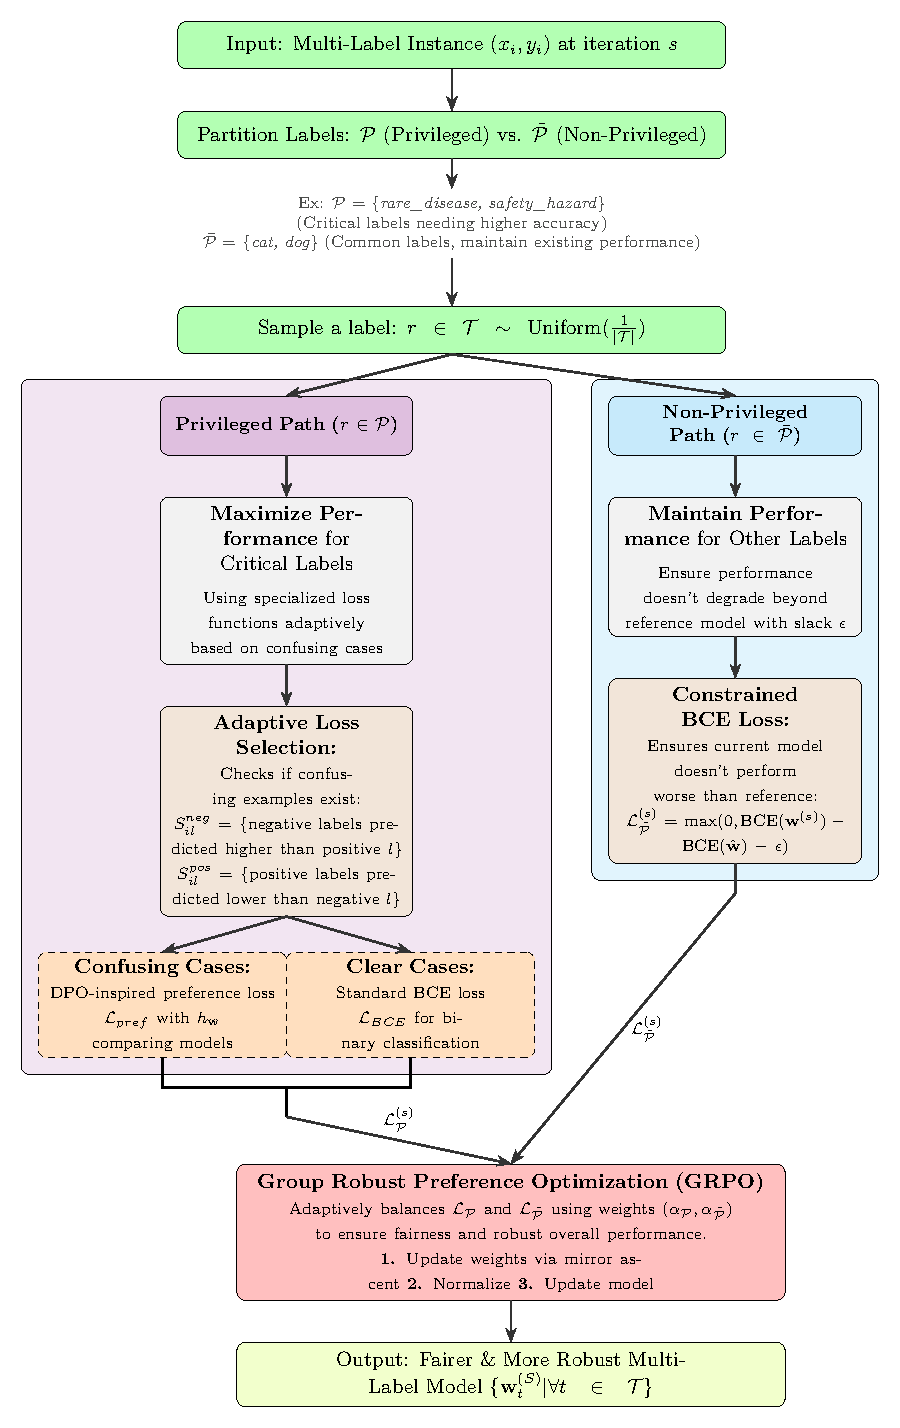
\includegraphics[width=0.5\linewidth]{Chapters/Chapter_5/method.pdf}
	\caption{Overview of the FairPO framework. Labels are partitioned into a
		privileged group and a non-privileged group. A sampled label is routed to the
		privileged path, which uses a preference loss with a BCE fallback, or the
		non-privileged path, which uses a constrained BCE loss against a reference
		model. A Group Robust Preference Optimization step balances the two group
		losses.}
	\label{fig:fairpo-overview}
\end{figure}

\subsection{Objective for the Privileged Group}
\label{subsec:fairpo-privileged}

For the privileged group, reweighting a standard loss is not enough. The main
difficulty for these labels is usually not basic classification but telling a label
apart from a close, incorrect alternative. We therefore set up the objective for
this group as a preference learning task.

\paragraph{Confusing counterparts.}
For an instance $\mathbf{x}_i$ and a privileged label $l \in \privileged$, we
identify a set of confusing counterparts from the model's current scores. There are
two cases. When the true label is positive ($y_{il}=1$), the confusing negatives
are the incorrect labels that the model scores at least as high as the true label:
\begin{equation}
	S_{il}^{\text{neg}} = \{k \in \labels \mid y_{ik}=0 \text{ and } \model(\mathbf{x}_i; \params_k) \ge \model(\mathbf{x}_i; \params_l) \}.
	\label{eq:fairpo-confusing-neg}
\end{equation}
When the true label is negative ($y_{il}=0$), the confusing positives are the
correct labels that the model scores no higher than the true negative:
\begin{equation}
	S_{il}^{\text{pos}} = \{k \in \labels \mid y_{ik}=1 \text{ and } \model(\mathbf{x}_i; \params_k) \le \model(\mathbf{x}_i; \params_l) \}.
	\label{eq:fairpo-confusing-pos}
\end{equation}
The full confusing set for $(i, l)$ is $\confusing = S_{il}^{\text{neg}} \cup S_{il}^{\text{pos}}$.

\paragraph{Conditional objective with a fallback.}
The objective for the privileged group is adaptive. When $\confusing$ is non-empty,
we apply a preference loss $\loss_{\text{pref}}$ to the hard discriminative case.
As the model improves, the confusing set for many instances becomes empty, and a
preference loss alone would then give a sparse gradient and stall training. To keep
a learning signal, we fall back to a standard binary cross-entropy loss when
$\confusing = \emptyset$:
\begin{equation}
	\baseloss_{\text{BCE}}(\mathbf{x}_i, y_{il}; \params_l) = -[y_{il} \log \model(\mathbf{x}_i; \params_l) + (1-y_{il}) \log(1-\model(\mathbf{x}_i; \params_l))].
	\label{eq:fairpo-bce}
\end{equation}
Early in training the model makes many mistakes, the confusing sets are large, and
the preference loss is used often. As the preference loss resolves these cases, the
fallback takes over and fine-tunes the easier examples. The total privileged loss
$\loss_{\privileged}$ is the expectation over this conditional choice.

\paragraph{DPO variant.}
To write the preference losses in one form, let $\model(\mathbf{x}_i; \params_p)$
be the score of the preferred label in a pair and
$\model(\mathbf{x}_i; \params_d)$ the score of the dispreferred label. The roles
follow the ground truth: if $y_{il}=1$ and $k \in S_{il}^{\text{neg}}$, then the
true label is preferred ($p=l$) and the confusing negative is dispreferred
($d=k$); if $y_{il}=0$ and $k \in S_{il}^{\text{pos}}$, then the true negative is
preferred ($p=l$) and the confusing positive is dispreferred ($d=k$). Following DPO
\citep{rafailov2023direct}, the preference loss is taken relative to the reference
model:
\begin{equation}
	\loss_{\text{pref}}^{\text{DPO}}(\mathbf{x}_i, p, d) = -\log \sigma \left( \beta \left( \log \frac{\model(\mathbf{x}_i; \params_p)}{\model(\mathbf{x}_i; \refparams_p)} - \log \frac{\model(\mathbf{x}_i; \params_d)}{\model(\mathbf{x}_i; \refparams_d)} \right) \right).
	\label{eq:fairpo-dpo-pref}
\end{equation}
The full DPO-based privileged loss combines this with the fallback:
\begin{align}
	\loss_{\privileged}^{\text{DPO}} = \E_{(\mathbf{x}_i,l) \text{ s.t. } l \in \privileged}
	\left[
	\mathbf{1}_{\confusing \neq \emptyset} \cdot \loss_{\text{pref}}^{\text{DPO}}(\mathbf{x}_i, p, d) + \mathbf{1}_{\confusing = \emptyset} \cdot \baseloss_{\text{BCE}}(\mathbf{x}_i, y_{il}; \params_l)
	\right],
	\label{eq:fairpo-dpo-combined}
\end{align}
where for a sampled privileged label $l$ with a non-empty confusing set, a
counterpart $k$ is sampled from $\confusing$ and the pair $(p,d)$ is set from
$(l,k)$ and the ground truth.

\paragraph{SimPO variant.}
This variant adapts SimPO \citep{meng2024simpo} to give
a reference-free preference loss with a target margin $\gamma > 0$, applied to the
per-label scores:
\begin{equation}
	\loss_{\text{pref}}^{\text{SimPO}}(\mathbf{x}_i, p, d) = -\log \sigma \left( \beta \log \frac{\model(\mathbf{x}_i; \params_p)}{\model(\mathbf{x}_i; \params_d)} - \gamma \right).
	\label{eq:fairpo-simpo-pref}
\end{equation}
The log-ratio term measures the relative preference, and the margin $-\gamma$ pushes
the model to separate the two scores by a set amount rather than only rank them
correctly. This term replaces the DPO term in the conditional objective of
Equation~\ref{eq:fairpo-dpo-combined}.

\paragraph{CPO variant.}
The last variant adapts CPO \citep{xu2024contrastive},
which is reference-free and adds a BCE regularizer to the preference term. When a
confusing set exists, the loss is
\begin{equation}
	\loss_{\text{pref}}^{\text{CPO}}(\mathbf{x}_i, p, d, l) = -\log \sigma \left( \beta \log \frac{\model(\mathbf{x}_i; \params_p)}{\model(\mathbf{x}_i; \params_d)} \right) + \lambda_{\text{CPO}} \cdot \baseloss_{\text{BCE}}(\mathbf{x}_i, y_{il}; \params_l).
	\label{eq:fairpo-cpo-pref}
\end{equation}
The first term is a margin-free preference objective, and the second, weighted by
$\lambda_{\text{CPO}}$, is the BCE loss for the privileged label $l$, which keeps
the model grounded in absolute scores. As in the DPO case, this loss is used when a
confusing set is found, and the BCE fallback of Equation~\ref{eq:fairpo-bce} is used
otherwise.

The reason for using a preference loss at all is that point-wise losses like BCE
and Focal Loss score each label on its own. They answer whether a label's score is
right in isolation, which gives only a weak signal when a true label at $0.8$ sits
just above a confusing label at $0.7$. The preference loss instead asks whether the
true label is scored clearly above its specific competitor, and the log-ratio gives
a direct gradient that pushes the two scores apart.

\subsection{Objective for the Non-Privileged Group}
\label{subsec:fairpo-nonprivileged}

For the non-privileged group the goal is not to push performance up but to keep it
from dropping. We use a constrained objective against the reference model. For a
label $j \in \nonprivileged$ we take the BCE loss of
Equation~\ref{eq:fairpo-bce}, and we penalize the model only when its loss is worse
than the reference model's loss by more than a slack margin $\epsilon \ge 0$,
through a hinge:
\begin{equation}
	\loss_{\nonprivileged} = \E_{(\mathbf{x}_i,j) \text{ s.t. } j \in \nonprivileged} \left[ \max(0, \baseloss_{\text{BCE}}(\mathbf{x}_i, y_{ij}; \params_j) - \baseloss_{\text{BCE}}(\mathbf{x}_i, y_{ij}; \refparams_j) - \epsilon) \right].
	\label{eq:fairpo-np-constrained}
\end{equation}
The gradient is zero as long as a non-privileged label is doing about as well as
the reference, and a signal appears only when the label drops below that threshold.
This keeps the non-privileged group from degrading while the model spends its
capacity on the privileged group.

\subsection{Group-Robust Balancing}
\label{subsec:fairpo-grpo}

We now have two objectives that pull against each other: the preference-based loss
$\loss_{\privileged}$ for the privileged group and the constrained loss
$\loss_{\nonprivileged}$ for the non-privileged group. A fixed weighted sum of the
two does not handle this well, since the right balance changes during training. We
instead treat the two label groups as the groups in a Group Robust Preference
Optimization problem \citep{ramesh2024group} and write the objective as a minimax
game:
\begin{equation}
	\min_{\{\params_t\}} \max_{\alpha \in \Delta} \left[ \alpha_{\privileged} \loss_{\privileged} + \alpha_{\nonprivileged} \loss_{\nonprivileged} \right],
	\label{eq:fairpo-objective}
\end{equation}
where $\alpha = (\alpha_{\privileged}, \alpha_{\nonprivileged})$ are adaptive
weights on the probability simplex $\Delta$. The inner maximization puts more
weight on whichever group currently has the higher loss, so training focuses on the
worse-off group, and the outer minimization updates the model under that weighting.
This gives a way to manage the trade-off between the two groups rather than fixing
it in advance.

\subsection{Optimization}
\label{subsec:fairpo-optim}

We solve Equation~\ref{eq:fairpo-objective} with alternating mirror ascent on the
weights $\alpha$ and mirror descent on the parameters $\params$, shown in
Algorithm~\ref{alg:fairpo-overview}. One detail matters for stability. The two
group losses can be on different scales, so using their raw values in the mirror
ascent step makes the weight updates unstable. We instead update $\alpha$ from the
change of each group's loss relative to its running average, which keeps the
balancing step stable.

\begin{algorithm}[t]
	\caption{FairPO Training Overview (DPO-inspired)}
	\label{alg:fairpo-overview}
	\begin{algorithmic}[1]
		\State \textbf{Initialize:} Model parameters $\Params^{(0)}$ (e.g., from supervised fine-tuning), group weights $\alpha_{\privileged}^{(0)}, \alpha_{\nonprivileged}^{(0)}$
		\State \textbf{Input:} Dataset $\dataset$, reference parameters $\Refparams$, hyperparameters $\beta, \epsilon, \eta_{\params}, \eta_{\alpha}$.
		\State \textbf{For} each training iteration $s = 0, \dots, S-1$:
		\State \hspace{0.5cm} Sample instance $(x_i, y_i) \sim \dataset$ and a label $r \in \mathcal{T}$.
		\State \hspace{0.5cm} \textbf{If} $r \in \privileged$:
		\State \hspace{1.0cm} Compute privileged loss $\loss_{\privileged}^{(s)}$ for $(x_i, r)$ (Eq.~\ref{eq:fairpo-dpo-combined}, or BCE Eq.~\ref{eq:fairpo-bce}).
		\State \hspace{0.5cm} \textbf{Else if} $r \in \nonprivileged$:
		\State \hspace{1.0cm} Compute non-privileged loss $\loss_{\nonprivileged}^{(s)}$ for $(x_i, r)$ (Eq.~\ref{eq:fairpo-np-constrained}).
		\State \hspace{0.5cm} Update group weights $\alpha^{(s+1)}$ via mirror ascent using $\loss_{\privileged}^{(s)}, \loss_{\nonprivileged}^{(s)}$.
		\State \hspace{0.5cm} Update model parameters $\Params^{(s+1)}$ via mirror descent using the weighted gradients.
		\State \textbf{End For}
		\State \textbf{Return} Optimized parameters $\Params^{(S)}$.
	\end{algorithmic}
\end{algorithm}

For the SimPO and CPO variants the structure is identical; only the preference term
inside the privileged loss changes, to
Equation~\ref{eq:fairpo-simpo-pref} or Equation~\ref{eq:fairpo-cpo-pref}. The
group-robust balancing and the non-privileged handling stay the same.


\section{Experimental Setup}
\label{sec:fairpo-setup}

\subsection{Datasets and Label Partition}
\label{subsec:fairpo-data}

We evaluate FairPO on two multi-label image benchmarks, MS-COCO~2014
\citep{lin2015coco} and NUS-WIDE \citep{chua2009nuswide}.
MS-COCO has 80 object categories, with 82{,}783 training images and 40{,}504
validation images, which we use as the test set. NUS-WIDE has 81 concept labels,
with 161{,}789 training images and 107{,}859 test images under the common split.

To set up the class-imbalance case, we partition the labels by frequency. On each
dataset the privileged group $\privileged$ is the set of 16 least frequent labels,
which is about $20\%$ of the labels, and the non-privileged group
$\nonprivileged$ is the rest, 64 labels on MS-COCO and 65 on NUS-WIDE. This makes
the rare labels the ones we try to improve and the frequent labels the ones we try
to maintain. The partition is one choice; as noted in
Section~\ref{subsec:fairpo-setup}, the framework allows other criteria, such as
domain importance.

\subsection{Model}
\label{subsec:fairpo-model}

The base model is a Vision Transformer, \texttt{vit-base-patch16-224}
\citep{dosovitskiy2021vit}, pre-trained on ImageNet-21k and
fine-tuned on ImageNet-1k. We keep the backbone frozen except for its final encoder
layer, which we leave trainable so the higher-level features can adapt. On top of
the backbone, each label has its own non-linear MLP head that takes the
$768$-dimensional feature from the ViT [CLS] token and outputs a single logit,
passed through a sigmoid to give the per-label score $\model(\mathbf{x}_i;
\params_t)$. Each head has the layer sizes $768 \rightarrow 256 \rightarrow 64
\rightarrow 16 \rightarrow 4 \rightarrow 1$ with ReLU activations between layers,
and the heads are independent across labels.

\subsection{Baselines and Variants}
\label{subsec:fairpo-baselines}

We compare against three baselines. BCE-SFT trains the same model with binary
cross-entropy; this is also the reference model $\refparams$ used by the FairPO
objectives. Group DRO + BCE \citep{sagawa2020dro} applies
distributionally robust optimization over label groups with a BCE loss. Focal Loss
\citep{lin2018focallossdenseobject} down-weights easy examples. We report the three
FairPO variants from Section~\ref{sec:fairpo-framework}: FairPO-DPO, FairPO-SimPO,
and FairPO-CPO.

\subsection{Metrics and Implementation}
\label{subsec:fairpo-impl}

We report mean average precision (mAP), Sample F1, and Accuracy, each split into the
privileged group $\privileged$ and the non-privileged group $\nonprivileged$. The
main quantity of interest is $\Delta\text{mAP}(\privileged)$, the change in mAP on
the privileged group relative to a baseline. All trainable parameters are updated
with AdamW \citep{loshchilov2019decoupled}. We train for at
most 25 epochs with a batch size of 32, with early stopping on validation mAP using
a patience of 5 epochs. Images are resized to $224 \times 224$, normalized with
ImageNet statistics, and augmented with random horizontal flips and random resized
crops. Each result is the mean over three runs.

\section{Results}
\label{sec:fairpo-results}

Tables~\ref{tab:fairpo-coco} and~\ref{tab:fairpo-nuswide} report the results on
MS-COCO and NUS-WIDE. Across both datasets, FairPO-CPO gives the best performance on
the privileged group. On MS-COCO it improves $\Delta\text{mAP}(\privileged)$ by
$+1.41$ over the strongest baseline (Focal Loss) and by $+3.44$ over BCE-SFT, and
the gain over the baselines is statistically significant. At the same time the drop
on the non-privileged group is small and not statistically significant
($-0.31$ relative to BCE-SFT). The same pattern holds on NUS-WIDE, where FairPO-CPO
gives the best privileged-group mAP with a non-privileged drop that is again small
and not significant. This is the behaviour the framework is designed for: the model
shifts capacity towards the rare labels without measurably hurting the frequent
ones.

The three variants do not behave the same way. FairPO-DPO improves the privileged
group but with a larger non-privileged drop than CPO. FairPO-SimPO is the weakest of
the three, falling below the baselines on the privileged group on both datasets.
FairPO-CPO is the most effective. The likely reason is its design: unlike DPO it is
reference-free, and unlike SimPO it includes a BCE regularizer that gives the model
a signal for absolute correctness alongside the relative preference. Learning both
the relative ranking and the absolute score makes its training more stable and is
what makes the CPO variant the most practical choice.

% TABLE 5.2 (MS-COCO main results) -- the paper's Table 1.
% Label: tab:fairpo-coco
\begin{table}[t]
	\caption{Performance comparison on MS-COCO. $\privileged$ is the privileged label
		set (20\% least frequent), and $\nonprivileged$ is the non-privileged set
		(remaining 80\%). Results are mean $\pm$ std.\ dev.\ over 3 runs. The best result
		for each metric is in \textbf{bold}. $\Delta$mAP is computed relative to the
		strongest baseline for each group (Focal Loss for $\privileged$, BCE-SFT for
		$\nonprivileged$). $^{\dagger}$ marks a statistically significant improvement
		($p<0.05$); $^{\ddagger}$ marks a difference that is not significant ($p>0.1$).}
	\label{tab:fairpo-coco}
	\centering
	\small
	\adjustbox{max width=\textwidth}{%
		\begin{tabular}{lcccccccc}
			\toprule
			\multicolumn{1}{c}{Method} & \multicolumn{2}{c}{mAP} & \multicolumn{2}{c}{Sample F1} & \multicolumn{2}{c}{Accuracy} & \multicolumn{1}{c}{$\Delta$ mAP ($\privileged$)} & \multicolumn{1}{c}{$\Delta$ mAP ($\nonprivileged$)} \\
			\cmidrule(lr){2-3} \cmidrule(lr){4-5} \cmidrule(lr){6-7}
			& $\privileged$ & $\nonprivileged$ & $\privileged$ & $\nonprivileged$ & $\privileged$ & $\nonprivileged$ & (vs.\ Focal) & (vs.\ BCE) \\
			\midrule
			BCE-SFT \citep{bce_loss}                       & 86.32$_{\pm 0.11}$ & \textbf{90.65}$_{\pm 0.08}$ & 61.43$_{\pm 0.15}$ & \textbf{64.89}$_{\pm 0.12}$ & 94.89$_{\pm 0.09}$ & \textbf{98.12}$_{\pm 0.05}$ & -2.03 & Ref \\
			GDRO + BCE \citep{sagawa2020dro}  & 87.92$_{\pm 0.12}$ & 90.41$_{\pm 0.09}$ & 62.31$_{\pm 0.20}$ & 64.75$_{\pm 0.13}$ & 95.72$_{\pm 0.10}$ & 98.05$_{\pm 0.05}$ & -0.43 & -0.24$^{\ddagger}$ \\
			Focal Loss \citep{lin2018focal} & 88.35$_{\pm 0.14}$ & 89.81$_{\pm 0.12}$ & 63.15$_{\pm 0.16}$ & 64.18$_{\pm 0.15}$ & 96.11$_{\pm 0.12}$ & 97.90$_{\pm 0.07}$ & Ref   & -0.84 \\
			\midrule
			FairPO-DPO                                     & 88.02$_{\pm 0.15}$ & 89.97$_{\pm 0.11}$ & 63.45$_{\pm 0.17}$ & 63.65$_{\pm 0.16}$ & 97.89$_{\pm 0.13}$ & 98.04$_{\pm 0.06}$ & -0.33 & -0.68 \\
			FairPO-SimPO                                   & 87.67$_{\pm 0.18}$ & 88.76$_{\pm 0.21}$ & 62.34$_{\pm 0.22}$ & 63.12$_{\pm 0.19}$ & 95.69$_{\pm 0.15}$ & 97.78$_{\pm 0.09}$ & -0.68 & -1.89 \\
			FairPO-CPO                                     & \textbf{89.76}$_{\pm 0.09}$ & 90.34$_{\pm 0.07}$ & \textbf{64.01}$_{\pm 0.13}$ & 64.32$_{\pm 0.10}$ & \textbf{98.03}$_{\pm 0.07}$ & 98.06$_{\pm 0.05}$ & \textbf{+1.41}$^{\dagger}$ & \textbf{-0.31}$^{\ddagger}$ \\
			\bottomrule
		\end{tabular}
	}
\end{table}

% TABLE 5.3 (NUS-WIDE main results) -- the paper's Table 2.
% Label: tab:fairpo-nuswide
\begin{table}[t]
	\caption{Performance comparison on NUS-WIDE. Notation is the same as
		Table~\ref{tab:fairpo-coco}.}
	\label{tab:fairpo-nuswide}
	\centering
	\small
	\adjustbox{max width=\textwidth}{%
		\begin{tabular}{lcccccccc}
			\toprule
			\multicolumn{1}{c}{Method} & \multicolumn{2}{c}{mAP} & \multicolumn{2}{c}{Sample F1} & \multicolumn{2}{c}{Accuracy} & \multicolumn{1}{c}{$\Delta$ mAP ($\privileged$)} & \multicolumn{1}{c}{$\Delta$ mAP ($\nonprivileged$)} \\
			\cmidrule(lr){2-3} \cmidrule(lr){4-5} \cmidrule(lr){6-7}
			& $\privileged$ & $\nonprivileged$ & $\privileged$ & $\nonprivileged$ & $\privileged$ & $\nonprivileged$ & (vs.\ Focal) & (vs.\ BCE) \\
			\midrule
			BCE-SFT \citep{bce_loss}                       & 63.53$_{\pm 0.15}$ & \textbf{70.24}$_{\pm 0.11}$ & 48.12$_{\pm 0.21}$ & \textbf{55.83}$_{\pm 0.14}$ & 91.51$_{\pm 0.12}$ & \textbf{95.22}$_{\pm 0.08}$ & -2.28 & Ref \\
			GDRO + BCE \citep{sagawa2020dro}  & 64.84$_{\pm 0.16}$ & 69.91$_{\pm 0.12}$ & 49.13$_{\pm 0.22}$ & 55.62$_{\pm 0.15}$ & 92.11$_{\pm 0.13}$ & 95.13$_{\pm 0.09}$ & -0.97 & -0.33 \\
			Focal Loss \citep{lin2018focal} & 65.81$_{\pm 0.17}$ & 68.95$_{\pm 0.15}$ & 50.33$_{\pm 0.20}$ & 54.31$_{\pm 0.18}$ & 93.05$_{\pm 0.11}$ & 94.75$_{\pm 0.11}$ & Ref   & -1.29 \\
			\midrule
			FairPO-DPO                                     & 66.34$_{\pm 0.20}$ & 69.05$_{\pm 0.14}$ & 51.71$_{\pm 0.25}$ & 54.52$_{\pm 0.19}$ & 93.92$_{\pm 0.16}$ & 95.04$_{\pm 0.09}$ & +0.53 & -1.19 \\
			FairPO-SimPO                                   & 64.11$_{\pm 0.22}$ & 68.03$_{\pm 0.24}$ & 48.82$_{\pm 0.28}$ & 53.81$_{\pm 0.22}$ & 91.94$_{\pm 0.18}$ & 94.52$_{\pm 0.13}$ & -1.70 & -2.21 \\
			FairPO-CPO                                     & \textbf{67.12}$_{\pm 0.14}$ & 69.83$_{\pm 0.10}$ & \textbf{52.21}$_{\pm 0.19}$ & 55.24$_{\pm 0.13}$ & \textbf{94.31}$_{\pm 0.10}$ & 95.12$_{\pm 0.08}$ & \textbf{+1.31}$^{\dagger}$ & \textbf{-0.41}$^{\ddagger}$ \\
			\bottomrule
		\end{tabular}
	}
\end{table}

\section{Ablation Studies}
\label{sec:fairpo-ablation}

We run ablations on MS-COCO with FairPO-CPO to check that each part of the framework
matters. Tables~\ref{tab:fairpo-ablation-core} and~\ref{tab:fairpo-ablation-pref}
report the results, with $\Delta\text{mAP}(\privileged)$ measured against BCE-SFT and
the parenthesized values showing the change relative to the full FairPO-CPO model.

Table~\ref{tab:fairpo-ablation-core} removes one component at a time. Replacing the
preference loss with BCE drops the privileged gain from $+3.44$ to $+1.80$, so the
preference signal accounts for much of the improvement. Removing the non-privileged
constraint keeps the privileged gain close ($+3.23$) but lets the non-privileged
group degrade, which defeats the purpose of the framework. Fixing the group weights
at $0.5/0.5$ instead of using the adaptive balancing lowers the privileged gain to
$+2.16$, showing that the balancing step is doing real work. A Global CPO variant
that applies the preference loss to all labels with no privileged/non-privileged
split reaches only $+2.23$, which is better than BCE but well short of the full
model, so the targeted partition matters.

Table~\ref{tab:fairpo-ablation-pref} looks at the preference objective itself.
Restricting the preference signal to only confusing negatives, and dropping the
confusing positives, is the most damaging change: the privileged gain falls to
$-13.17$, a large drop, because the model loses the signal that handles
true-negative labels with confusing positives. Removing the BCE fallback for the
non-confusing case lowers the gain from $+3.44$ to $+2.73$, which confirms that the
fallback is needed to keep a stable signal once the confusing sets empty out. Taken
together, the ablations show that the gain comes from the complete framework, not
from any single piece.

% TABLE 5.4 (ablation: core components) -- the paper's Table 3.
% Label: tab:fairpo-ablation-core
\begin{table}[h]
	\caption{Ablation on the core components of FairPO-CPO (MS-COCO).
		$\Delta\text{mAP}(\privileged)$ is measured against BCE-SFT. Parentheses show the
		change relative to the full FairPO-CPO model.}
	\label{tab:fairpo-ablation-core}
	\centering
	\tiny
	\adjustbox{max width=\textwidth}{%
		\begin{tabular}{lccccccc}
			\toprule
			\multicolumn{1}{c}{Method Variant} & \multicolumn{2}{c}{mAP} & \multicolumn{2}{c}{Sample F1} & \multicolumn{2}{c}{Accuracy} & \multicolumn{1}{c}{$\Delta\text{mAP}(\privileged)$} \\
			\cmidrule(lr){2-3} \cmidrule(lr){4-5} \cmidrule(lr){6-7}
			& $\privileged$ & $\nonprivileged$ & $\privileged$ & $\nonprivileged$ & $\privileged$ & $\nonprivileged$ & \\
			\midrule
			FairPO-CPO (Full)                  & \textbf{89.76} & \textbf{90.34} & \textbf{64.01} & \textbf{64.32} & \textbf{98.03} & \textbf{98.06} & \textbf{+3.44} \\
			\midrule
			\textit{w/o Preference Loss}       & 88.12          & 90.45          & 62.45          & 64.80          & 95.80          & 98.09          & +1.80 \\
			($\loss_{\privileged}$ is BCE)     & (-1.64)        & (+0.11)        & (-1.56)        & (+0.48)        & (-2.23)        & (+0.03)        & \\
			\midrule
			\textit{w/o $\nonprivileged$ Constraint} & 89.55    & 88.98          & 63.70          & 62.95          & 97.90          & 97.55          & +3.23 \\
			($\loss_{\nonprivileged}$ is BCE)  & (-0.21)        & (-1.36)        & (-0.31)        & (-1.37)        & (-0.13)        & (-0.51)        & \\
			\midrule
			\textit{w/o GRPO}                  & 88.48          & 89.75          & 62.88          & 63.50          & 96.53          & 97.88          & +2.16 \\
			(Fixed 0.5/0.5 weights)            & (-1.28)        & (-0.59)        & (-1.13)        & (-0.82)        & (-1.50)        & (-0.18)        & \\
			\midrule
			\textit{Global CPO (all labels)}   & 88.55          & 90.68          & 62.75          & 64.85          & 96.95          & 98.11          & +2.23 \\
			(No $\privileged$/$\nonprivileged$ split) & (-1.21) & (+0.34)        & (-1.26)        & (+0.47)        & (-1.08)        & (+0.05)        & \\
			\bottomrule
		\end{tabular}
	}
\end{table}

% TABLE 5.5 (ablation: preference formulation) -- the paper's Table 4.
% Label: tab:fairpo-ablation-pref
\begin{table}[h]
	\caption{Ablation on the preference formulation (FairPO-CPO, MS-COCO).
		$\Delta\text{mAP}(\privileged)$ is measured against BCE-SFT. Parentheses show the
		change relative to the full FairPO-CPO model.}
	\label{tab:fairpo-ablation-pref}
	\centering
	\tiny
	\adjustbox{max width=\textwidth}{%
		\begin{tabular}{lccccccc}
			\toprule
			\multicolumn{1}{c}{Preference Detail Variant} & \multicolumn{2}{c}{mAP} & \multicolumn{2}{c}{Sample F1} & \multicolumn{2}{c}{Accuracy} & \multicolumn{1}{c}{$\Delta\text{mAP}(\privileged)$} \\
			\cmidrule(lr){2-3} \cmidrule(lr){4-5} \cmidrule(lr){6-7}
			& $\privileged$ & $\nonprivileged$ & $\privileged$ & $\nonprivileged$ & $\privileged$ & $\nonprivileged$ & \\
			\midrule
			FairPO-CPO (Full)                  & \textbf{89.76} & \textbf{90.34} & \textbf{64.01} & \textbf{64.32} & \textbf{98.03} & \textbf{98.06} & \textbf{+3.44} \\
			(Conf.\ Neg \& Pos, BCE Fallback)  &                &                &                &                &                &                & \\
			\midrule
			\textit{Only Confusing Negatives}  & 73.15          & 90.25          & 47.88          & 64.20          & 94.67          & 98.01          & -13.17 \\
			& (-16.61)       & (-0.09)        & (-16.13)       & (-0.12)        & (-3.36)        & (-0.05)        & \\
			\midrule
			\textit{w/o BCE Fallback}          & 89.05          & 90.21          & 63.20          & 64.10          & 97.55          & 97.99          & +2.73 \\
			(No loss if $\confusing=\emptyset$) & (-0.71)       & (-0.13)        & (-0.81)        & (-0.22)        & (-0.48)        & (-0.07)        & \\
			\bottomrule
		\end{tabular}
	}
\end{table}

\section{Discussion and Limitations}
\label{sec:fairpo-discussion}

FairPO shows that an objective can be designed to improve a chosen group of labels
while protecting the rest. The preference loss gives the privileged group a signal
that point-wise losses do not, the constrained objective keeps the non-privileged
group from degrading, and the group-robust balancing manages the trade-off between
them. The results bear out the larger point of the thesis: the useful place to act
is the training objective. Where Chapter~\ref{ch:neurons} found that editing a
small set of internal components did not reallocate a model's behaviour, here a
change at the level of the objective does, improving the rare labels without
measurable harm to the frequent ones.

The framework has limitations. The confusing set is computed from the model's
current scores and changes during training, which can make it unstable. The DPO
variant needs a reference model, which the CPO and SimPO variants avoid. The
group-robust balancing has hyperparameters that need care, since the two losses are
on different scales and the balancing step has to be stabilized through loss
scaling. The experiments here use a frequency-based label partition on two image
benchmarks; other partition criteria and other domains are left for future work,
along with extending the approach beyond classification.

